\documentclass[tikz, border=10pt]{standalone}
\begin{document}

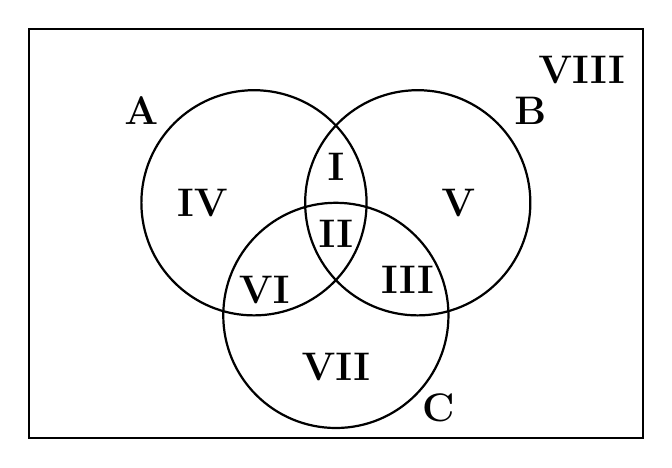
\begin{tikzpicture}[scale=1.3]
    % Draw the universal set rectangle
    \draw[thick] (-2.2,-2) rectangle (3.8,2);
    
    % Draw three circles
    \draw[thick] (0,0.3) circle (1.1cm);
    \draw[thick] (1.6,0.3) circle (1.1cm);
    \draw[thick] (0.8,-0.8) circle (1.1cm);
    
    % Label the sets
    \node at (-1.1,1.2) {\Large \textbf{A}};
    \node at (2.7,1.2) {\Large \textbf{B}};
    \node at (1.8,-1.7) {\Large \textbf{C}};
    
    % Label the regions with Roman numerals
    \node at (-0.5,0.3) {\Large \textbf{IV}};
    \node at (0.8,0.65) {\Large \textbf{I}};
    \node at (0.8,0) {\Large \textbf{II}};
    \node at (1.5,-0.45) {\Large \textbf{III}};
    \node at (2,0.3) {\Large \textbf{V}};
    \node at (0.1,-0.55) {\Large \textbf{VI}};
    \node at (0.8,-1.3) {\Large \textbf{VII}};
    \node at (3.2,1.6) {\Large \textbf{VIII}};
\end{tikzpicture}

\end{document}
